%iffalse
\let\negmedspace\undefined
\let\negthickspace\undefined
\documentclass[journal,12pt,onecolumn]{IEEEtran}
\usepackage{cite}
\usepackage{amsmath,amssymb,amsfonts,amsthm}
\usepackage{algorithmic}
\usepackage{graphicx}
\usepackage{textcomp}
\usepackage{xcolor}
\usepackage{txfonts}
\usepackage{listings}
\usepackage{enumitem}
\usepackage{mathtools}
\usepackage{gensymb}
\usepackage{comment}
\usepackage[breaklinks=true]{hyperref}
\usepackage{tkz-euclide} 
\usepackage{circuitikz}
\usepackage{listings}
\usepackage{gvv}      
%\def\inputGnumericTable{} 

\newcommand{\tripleprime}{{\prime\prime\prime}}



\usepackage{tikz}
\usepackage[latin1]{inputenc} 

\usepackage{caption}
\usepackage{subcaption}

\usepackage{color}                                            
\usepackage{array}                                            
\usepackage{longtable}                                       
\usepackage{calc}                                             
\usepackage{multirow}    
\usepackage{hhline}                                           
\usepackage{ifthen}     
\usepackage{tikz}
\usepackage{lscape}
\usepackage{tabularx}
\usepackage{array}
\usepackage{float}
\usepackage{multicol}
\usetikzlibrary{patterns}



\newtheorem{theorem}{Theorem}[section]
\newtheorem{problem}{Problem}
\newtheorem{proposition}{Proposition}[section]
\newtheorem{lemma}{Lemma}[section]
\newtheorem{corollary}[theorem]{Corollary}
\newtheorem{example}{Example}[section]
\newtheorem{definition}[problem]{Definition}
\newcommand{\BEQA}{\begin{eqnarray}}
\newcommand{\EEQA}{\end{eqnarray}}
\newcommand{\define}{\stackrel{\triangle}{=}}
\theoremstyle{remark}
\newtheorem{rem}{Remark}

% Marks the beginning of the document
\begin{document}
\bibliographystyle{IEEEtran}
\vspace{3cm}

\title{CE : GATE 2020}
\author{ai24btech11014 \\ Charitha Sri}

\maketitle
\bigskip       
\renewcommand{\thefigure}{\theenumi}
\renewcommand{\thetable}{\theenumi}

\section{27-39}
\begin{enumerate}
\item A continuous function $f\brak{x}$ is defined. If the third derivative at $x_{i}$ is to be computed by using the fourth order central finite-divided-difference scheme (with step length = $h$), the correct formula is 
\begin{enumerate}
    \item $f^{\tripleprime} \brak{x_{i}} = \frac{-f\brak{x_{i+3}} + 8 f\brak{x_{i+ 2}} -13 f \brak{x_{i+ 1}} + 13f\brak{x_{i-1}} - 8 f\brak{x_{i-2}} + f\brak{x_{i - 3}}}{8 h ^{3}}$
\\
     \item $f^{\tripleprime} \brak{x_{i}} = \frac{f\brak{x_{i+3}} - 8 f\brak{x_{i+ 2}} -13 f \brak{x_{i+ 1}} + 13f\brak{x_{i-1}} + 8 f\brak{x_{i-2}} + f\brak{x_{i - 3}}}{8 h ^{3}}$
\\
     \item $f^{\tripleprime} \brak{x_{i}} = \frac{-f\brak{x_{i+3}} - 8 f\brak{x_{i+ 2}} -13 f \brak{x_{i+ 1}} + 13f\brak{x_{i-1}} + 8 f\brak{x_{i-2}} - f\brak{x_{i - 3}}}{8 h ^{3}}$
\\
     \item $f^{\tripleprime} \brak{x_{i}} = \frac{f\brak{x_{i+3}} - 8 f\brak{x_{i+ 2}} + 13 f \brak{x_{i+ 1}} + 13f\brak{x_{i-1}} - 8 f\brak{x_{i-2}} - f\brak{x_{i - 3}}}{8 h ^{3}}$  
\end{enumerate}

\item Distributed load(s) 0f $ 50 k N/m $ may occupy any position(s) (either continuously or in patches) on the grider $\textbf{PQRST}$ as shown in the figure (not drawn to the scale)
The maximum negative negative (hogging) bending moment (in $k N. m$) that occurs at point R, is 
\begin{center}

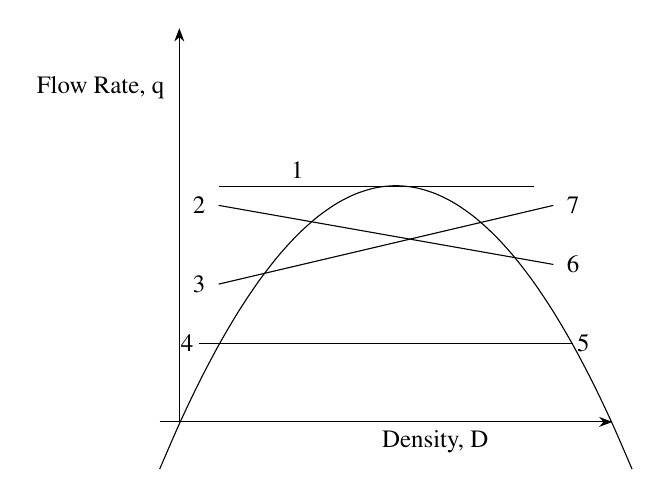
\begin{tikzpicture}

% Arrows for flow
\draw [->, >=Stealth] (6,9.5) -- (11.75,9.5);
\draw [->, >=Stealth] (6.25,9.5) -- (6.25,14.5);

% Labels for density and flow rate
\node [font=\small] at (9.5,9.25) {Density, D};
\node [font=\small] at (5.25,13.75) {Flow Rate, q};

% Short lines representing segments
\draw [-] (6.75,12.49) -- (10.75,12.49);
\draw [-] (6.75,11.25) -- (11,12.25);
\draw [-] (6.75,12.25) -- (11,11.5);
\draw [-] (6.5,10.5) -- (11.25,10.5);

% Labels for points
\node [font=\small] at (7.75,12.7) {1};
\node [font=\small] at (6.5,12.25) {2};
\node [font=\small] at (11.25,12.25) {7};
\node [font=\small] at (6.5,11.25) {3};
\node [font=\small] at (11.25,11.5) {6};
\node [font=\small] at (11.38,10.5) {5};
\node [font=\small] at (6.35,10.5) {4};

% Downward-opening parabola that passes through (6.5, 9.5) and (11.5, 9.5)
\draw[domain=6:12,smooth,variable=\x,black] plot (\x,{-(0.4*(\x - 9)^2) + 12.5}); 


\end{tikzpicture}


\end{center}
\begin{enumerate}
\begin{multicols}{4}
    \item $22.50$
    \item $56.25$
    \item $93.75$
    \item $150.00$
\end{multicols}
\end{enumerate}
\item A rigid weightless platform $\textbf{PQRS}$ shown in the figure (not drawn to the scale)  can slide freely in the vertical direction. The platform is held in position by the weightless member $\textbf{OJ}$ and four weightless, frictionless rollers. Points $\textbf{O}$ and $ \textbf{J} $ are pin connections. A block of $90 kN $ rests on the platform as shown in the figure
The magnitude of horizontal componenet of the reaction (in $kN$) at pin $\textbf{O}$, is 

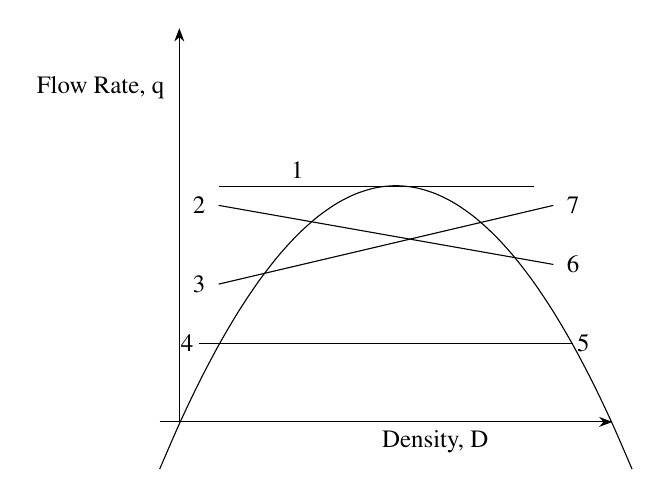
\begin{tikzpicture}

% Arrows for flow
\draw [->, >=Stealth] (6,9.5) -- (11.75,9.5);
\draw [->, >=Stealth] (6.25,9.5) -- (6.25,14.5);

% Labels for density and flow rate
\node [font=\small] at (9.5,9.25) {Density, D};
\node [font=\small] at (5.25,13.75) {Flow Rate, q};

% Short lines representing segments
\draw [-] (6.75,12.49) -- (10.75,12.49);
\draw [-] (6.75,11.25) -- (11,12.25);
\draw [-] (6.75,12.25) -- (11,11.5);
\draw [-] (6.5,10.5) -- (11.25,10.5);

% Labels for points
\node [font=\small] at (7.75,12.7) {1};
\node [font=\small] at (6.5,12.25) {2};
\node [font=\small] at (11.25,12.25) {7};
\node [font=\small] at (6.5,11.25) {3};
\node [font=\small] at (11.25,11.5) {6};
\node [font=\small] at (11.38,10.5) {5};
\node [font=\small] at (6.35,10.5) {4};

% Downward-opening parabola that passes through (6.5, 9.5) and (11.5, 9.5)
\draw[domain=6:12,smooth,variable=\x,black] plot (\x,{-(0.4*(\x - 9)^2) + 12.5}); 


\end{tikzpicture}


\begin{enumerate}
\begin{multicols}{4}
\item $90$
\item $ 120$
\item $ 150$
\item $ 180 $
\end{multicols}
\end{enumerate}

\item A cantilever beam $\textbf{PQ}$ of uniform flexural rigidity ($EI$) is subjected to a concentrated moment M at $\textbf{R}$ as shown in the figure



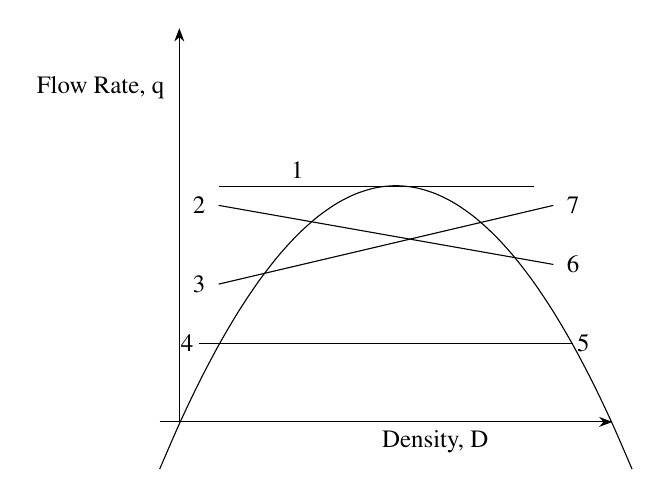
\begin{tikzpicture}

% Arrows for flow
\draw [->, >=Stealth] (6,9.5) -- (11.75,9.5);
\draw [->, >=Stealth] (6.25,9.5) -- (6.25,14.5);

% Labels for density and flow rate
\node [font=\small] at (9.5,9.25) {Density, D};
\node [font=\small] at (5.25,13.75) {Flow Rate, q};

% Short lines representing segments
\draw [-] (6.75,12.49) -- (10.75,12.49);
\draw [-] (6.75,11.25) -- (11,12.25);
\draw [-] (6.75,12.25) -- (11,11.5);
\draw [-] (6.5,10.5) -- (11.25,10.5);

% Labels for points
\node [font=\small] at (7.75,12.7) {1};
\node [font=\small] at (6.5,12.25) {2};
\node [font=\small] at (11.25,12.25) {7};
\node [font=\small] at (6.5,11.25) {3};
\node [font=\small] at (11.25,11.5) {6};
\node [font=\small] at (11.38,10.5) {5};
\node [font=\small] at (6.35,10.5) {4};

% Downward-opening parabola that passes through (6.5, 9.5) and (11.5, 9.5)
\draw[domain=6:12,smooth,variable=\x,black] plot (\x,{-(0.4*(\x - 9)^2) + 12.5}); 


\end{tikzpicture}


The deflection at the free end $\textbf{Q}$ is
\begin{enumerate}
\begin{multicols}{4}
\item $\frac{ML^{2}}{6 EI}$
\item $\frac{ML^{2}}{4 EI}$
\item $\frac{3 ML^{2}}{8 EI}$
\item $\frac{3 ML^{2}}{4 EI}$
\end{multicols}
\end{enumerate}

\item A dowel bar is placed at a contraction joint. When contraction occurs, the concrete slab cracks at predetermined location(s). Identify the arrangement, which shows the correct placement of dowel bar and the place of occurence of the contraction crack(s).

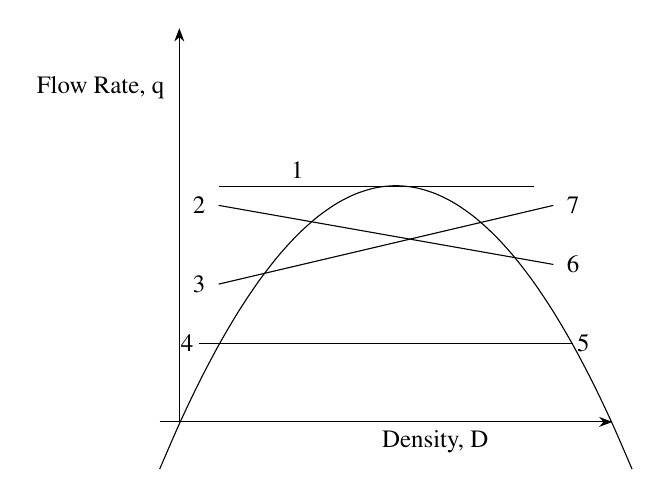
\begin{tikzpicture}

% Arrows for flow
\draw [->, >=Stealth] (6,9.5) -- (11.75,9.5);
\draw [->, >=Stealth] (6.25,9.5) -- (6.25,14.5);

% Labels for density and flow rate
\node [font=\small] at (9.5,9.25) {Density, D};
\node [font=\small] at (5.25,13.75) {Flow Rate, q};

% Short lines representing segments
\draw [-] (6.75,12.49) -- (10.75,12.49);
\draw [-] (6.75,11.25) -- (11,12.25);
\draw [-] (6.75,12.25) -- (11,11.5);
\draw [-] (6.5,10.5) -- (11.25,10.5);

% Labels for points
\node [font=\small] at (7.75,12.7) {1};
\node [font=\small] at (6.5,12.25) {2};
\node [font=\small] at (11.25,12.25) {7};
\node [font=\small] at (6.5,11.25) {3};
\node [font=\small] at (11.25,11.5) {6};
\node [font=\small] at (11.38,10.5) {5};
\node [font=\small] at (6.35,10.5) {4};

% Downward-opening parabola that passes through (6.5, 9.5) and (11.5, 9.5)
\draw[domain=6:12,smooth,variable=\x,black] plot (\x,{-(0.4*(\x - 9)^2) + 12.5}); 


\end{tikzpicture}





\item The relationship between traffic flow rate (q) and density (D) is shown in the figure
	\begin{center}
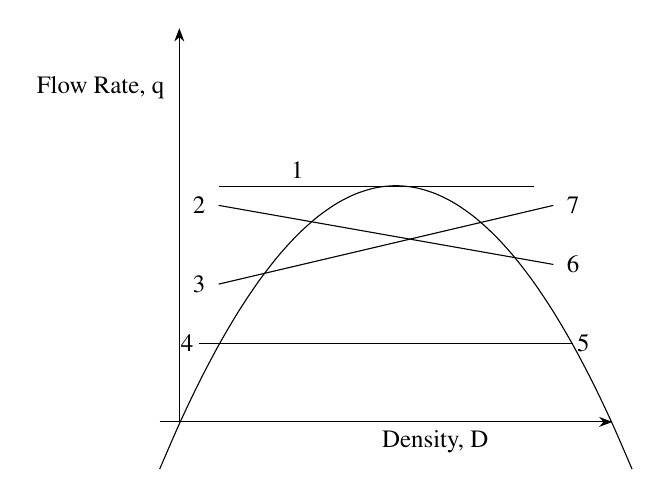
\begin{tikzpicture}

% Arrows for flow
\draw [->, >=Stealth] (6,9.5) -- (11.75,9.5);
\draw [->, >=Stealth] (6.25,9.5) -- (6.25,14.5);

% Labels for density and flow rate
\node [font=\small] at (9.5,9.25) {Density, D};
\node [font=\small] at (5.25,13.75) {Flow Rate, q};

% Short lines representing segments
\draw [-] (6.75,12.49) -- (10.75,12.49);
\draw [-] (6.75,11.25) -- (11,12.25);
\draw [-] (6.75,12.25) -- (11,11.5);
\draw [-] (6.5,10.5) -- (11.25,10.5);

% Labels for points
\node [font=\small] at (7.75,12.7) {1};
\node [font=\small] at (6.5,12.25) {2};
\node [font=\small] at (11.25,12.25) {7};
\node [font=\small] at (6.5,11.25) {3};
\node [font=\small] at (11.25,11.5) {6};
\node [font=\small] at (11.38,10.5) {5};
\node [font=\small] at (6.35,10.5) {4};

% Downward-opening parabola that passes through (6.5, 9.5) and (11.5, 9.5)
\draw[domain=6:12,smooth,variable=\x,black] plot (\x,{-(0.4*(\x - 9)^2) + 12.5}); 


\end{tikzpicture}

	\end{center}

The shock wave condition is depicted by 
\begin{enumerate}
\item flow with respect to point 1 $\brak{q_{1} = q_{max}}$
\item flow changing from point 2 to point 6 $\brak{q_{2} > q_{6}}$
\item flow changing from point 3 to point 7 $\brak{q_{3} < q_{7}}$
\item flow with respect to point 4 and point 5 $\brak{q_{4} = q_{5}}$
\end{enumerate}

\item The appropriate design length of a clearway is calculated on the basis of 'Normal Take-off' condition. Which one of the following options correctly depicts the length of the clearway? (Note: None of the options are drawn to scale )
	\begin{center}
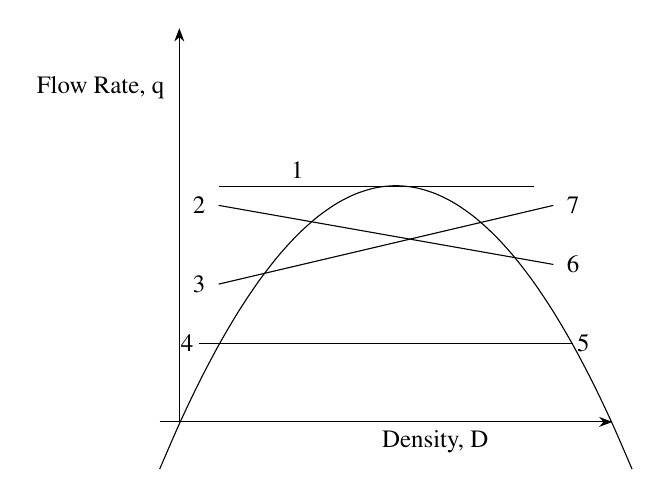
\begin{tikzpicture}

% Arrows for flow
\draw [->, >=Stealth] (6,9.5) -- (11.75,9.5);
\draw [->, >=Stealth] (6.25,9.5) -- (6.25,14.5);

% Labels for density and flow rate
\node [font=\small] at (9.5,9.25) {Density, D};
\node [font=\small] at (5.25,13.75) {Flow Rate, q};

% Short lines representing segments
\draw [-] (6.75,12.49) -- (10.75,12.49);
\draw [-] (6.75,11.25) -- (11,12.25);
\draw [-] (6.75,12.25) -- (11,11.5);
\draw [-] (6.5,10.5) -- (11.25,10.5);

% Labels for points
\node [font=\small] at (7.75,12.7) {1};
\node [font=\small] at (6.5,12.25) {2};
\node [font=\small] at (11.25,12.25) {7};
\node [font=\small] at (6.5,11.25) {3};
\node [font=\small] at (11.25,11.5) {6};
\node [font=\small] at (11.38,10.5) {5};
\node [font=\small] at (6.35,10.5) {4};

% Downward-opening parabola that passes through (6.5, 9.5) and (11.5, 9.5)
\draw[domain=6:12,smooth,variable=\x,black] plot (\x,{-(0.4*(\x - 9)^2) + 12.5}); 


\end{tikzpicture}

	\end{center}

\item The total stress paths corresponding to different loading conditions, for a soil specimen under the isotropically consolidated stress state(O), are shown below 

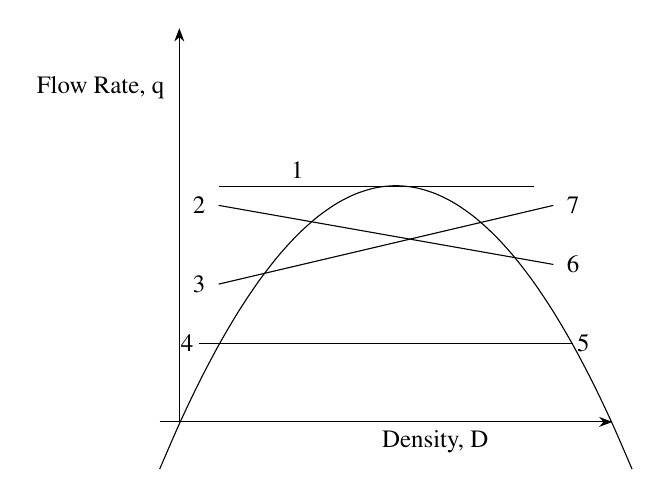
\begin{tikzpicture}

% Arrows for flow
\draw [->, >=Stealth] (6,9.5) -- (11.75,9.5);
\draw [->, >=Stealth] (6.25,9.5) -- (6.25,14.5);

% Labels for density and flow rate
\node [font=\small] at (9.5,9.25) {Density, D};
\node [font=\small] at (5.25,13.75) {Flow Rate, q};

% Short lines representing segments
\draw [-] (6.75,12.49) -- (10.75,12.49);
\draw [-] (6.75,11.25) -- (11,12.25);
\draw [-] (6.75,12.25) -- (11,11.5);
\draw [-] (6.5,10.5) -- (11.25,10.5);

% Labels for points
\node [font=\small] at (7.75,12.7) {1};
\node [font=\small] at (6.5,12.25) {2};
\node [font=\small] at (11.25,12.25) {7};
\node [font=\small] at (6.5,11.25) {3};
\node [font=\small] at (11.25,11.5) {6};
\node [font=\small] at (11.38,10.5) {5};
\node [font=\small] at (6.35,10.5) {4};

% Downward-opening parabola that passes through (6.5, 9.5) and (11.5, 9.5)
\draw[domain=6:12,smooth,variable=\x,black] plot (\x,{-(0.4*(\x - 9)^2) + 12.5}); 


\end{tikzpicture}



\begin{table}[h]
        \centering
        \begin{tabular}{ c@{\hskip 1cm }c }
            Group I & Group II \\
            P. Alidade & 1. Chain surveying \\
            Q. Arrow & 2. Levelling \\
            R. Bubble tube & 3. Plain table surveying \\
            S. Stadia hair & 4. Theodolite surveying \\
        \end{tabular}
    \end{table}




The correct match between the stress paths and the listed loading conditions, is 
\begin{enumerate}

\item OP-I, OQ-II, OR-1V, OS-III
\item OP-IV, OQ-III, OR-I, OS-II
\item OP-III, OQ-II, OR-I, OS-IV
\item OP-I, OQ-III, OR-II, OS-IV

\end{enumerate}

\item The soil profile at a site up to a depth of $10m $ is shown in the figure (not drawn to the scale ). The soil is preloaded with a uniform subcharge (q) of $70 kN/m^{2}$ at the ground level. The water table is at a depth of $3m $, below ground level. The soil unit weight of the respective layers is shown in the figure. Consider unit weight of water as $9.81 k N/m^{3}$ and assume that the surcharge (q) is applied instantaneously. Immediately after preloading, the effective stresses (in $kPa$) at points $P $ an $Q$, respectively, are

	\begin{center}
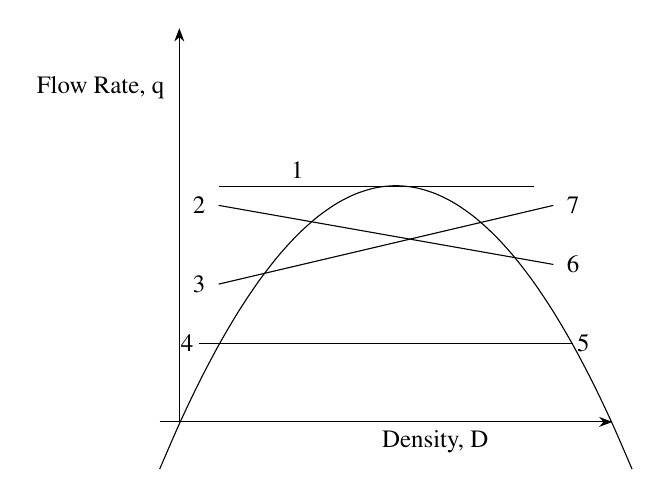
\begin{tikzpicture}

% Arrows for flow
\draw [->, >=Stealth] (6,9.5) -- (11.75,9.5);
\draw [->, >=Stealth] (6.25,9.5) -- (6.25,14.5);

% Labels for density and flow rate
\node [font=\small] at (9.5,9.25) {Density, D};
\node [font=\small] at (5.25,13.75) {Flow Rate, q};

% Short lines representing segments
\draw [-] (6.75,12.49) -- (10.75,12.49);
\draw [-] (6.75,11.25) -- (11,12.25);
\draw [-] (6.75,12.25) -- (11,11.5);
\draw [-] (6.5,10.5) -- (11.25,10.5);

% Labels for points
\node [font=\small] at (7.75,12.7) {1};
\node [font=\small] at (6.5,12.25) {2};
\node [font=\small] at (11.25,12.25) {7};
\node [font=\small] at (6.5,11.25) {3};
\node [font=\small] at (11.25,11.5) {6};
\node [font=\small] at (11.38,10.5) {5};
\node [font=\small] at (6.35,10.5) {4};

% Downward-opening parabola that passes through (6.5, 9.5) and (11.5, 9.5)
\draw[domain=6:12,smooth,variable=\x,black] plot (\x,{-(0.4*(\x - 9)^2) + 12.5}); 


\end{tikzpicture}

	\end{center}

\begin{enumerate}
\begin{multicols}{4}
\item $124$ and $204$
\item $ 36 $ and $ 90 $
\item $ 36 $ and $ 126 $
\item $ 54 $ and $95 $
\end{multicols}
\end{enumerate}

\item Water flow at the rate of $12 m^{3}/s $ in a $6m $ wide rectangular channel. A hydraulic jump is formed in the channel at a point where the upstream depth is  $ 30cm $ (just before the jump). Considering acceleration due to gravity as $9.81 m/s^{2}$ and density of water as $1000kg/m^{3}$, the energy loss in the jump is 
\begin{enumerate}
\begin{multicols}{4}
\item $114.2 k W$
\item $114.2 MW$
\item $141.2 h.p.$
\item $ 141.2 J/s $
\end{multicols}
\end{enumerate}

\item A water supply scheme transports scheme transports $10MLD$ (Million Litres per Day) water through a $450mm $ diameter pipeline for a distance of $2.5 km $. A chlorine dosee of $3.50 mg/litre$ is applied at the starting point of the pipeline to attain a certain level of disinfection at the downstream end. It is decided to increase the flow rate from $10 MLD$ to $13 MLD$ in the pipeline. Assume exponent for concentration, $n = 0.86 $.  With this increased flow, in oreder to attain the same level of disinfection, the chlorine dose (in mg/litre) to be applied at the starting point should be
\begin{enumerate}
\begin{multicols}{4}
\item $ 3.95 $
\item $ 4.40 $
\item $ 4.75 $
\item $ 5.55 $
\end{multicols}
\end{enumerate}

\item An open traverse $PQRST$ is surveyed using theodolite and the consecutive coordinates obtained are given in the table


\begin{table}[h]
        \centering
        \begin{tabular}{ c@{\hskip 1cm }c }
            Group I & Group II \\
            P. Alidade & 1. Chain surveying \\
            Q. Arrow & 2. Levelling \\
            R. Bubble tube & 3. Plain table surveying \\
            S. Stadia hair & 4. Theodolite surveying \\
        \end{tabular}
    \end{table}


If the independent coordinates (Northing, Easting) of station $P$ are $\brak{400m, 200m}$,
the independent coordinates (in m) of station $T$, are
\begin{enumerate}
\begin{multicols}{4}
\item $ 194.7, 370.1 $
\item $ 205.3, 429.9 $
\item $ 394.7, 170.1 $
\item $ 405.3, 229.9 $
\end{multicols}
\end{enumerate}

\item If $C$ represents a line segment between $\brak{0, 0, 0}$ and $\brak{1, 1, 1}$ in Cartesian coordinate system, the value (expresssed as integer) of the line integral 
\begin{align}
\int_{C} \sbrak{\brak{y + z} dx + \brak{ x+ z} dy + \brak{x + y} dz} 
\end{align}
is \underline{\hspace{2cm}}.

\end{enumerate}
\end{document}
